% Beamer Presentation
% LaTeX Template
% Version 1.0 (10/11/12)
%
% This template has been downloaded from:
% http://www.LaTeXTemplates.com
%
% License:
% CC BY-NC-SA 3.0 (http://creativecommons.org/licenses/by-nc-sa/3.0/)
%
%%%%%%%%%%%%%%%%%%%%%%%%%%%%%%%%%%%%%%%%%

%----------------------------------------------------------------------------------------
%	PACKAGES AND THEMES
%----------------------------------------------------------------------------------------


\documentclass[xcolor=dvipsnames]{beamer}

\mode<presentation> {

% The Beamer class comes with a number of default slide themes
% which change the colors and layouts of slides. Below this is a list
% of all the themes, uncomment each in turn to see what they look like.

\usetheme{PaloAlto}

% As well as themes, the Beamer class has a number of color themes
% for any slide theme. Uncomment each of these in turn to see how it
% changes the colors of your current slide theme.

\usecolortheme{dove}

%\setbeamertemplate{footline} % To remove the footer line in all slides uncomment this line
%\setbeamertemplate{footline}[page number] % To replace the footer line in all slides with a simple slide count uncomment this line

%\setbeamertemplate{navigation symbols}{} % To remove the navigation symbols from the bottom of all slides uncomment this line
}

\usepackage[spanish]{babel}
\usepackage[utf8]{inputenc}

\usepackage{graphicx} % Allows including images
\usepackage{booktabs} % Allows the use of \toprule, \midrule and \bottomrule in tables
\usepackage{multimedia}
\usepackage{wrapfig}
\usepackage{multicol}
\usepackage{vwcol}
\usepackage[export]{adjustbox}

\usepackage{color}
\definecolor{gray97}{gray}{.97}
\definecolor{gray75}{gray}{.75}
\definecolor{gray45}{gray}{.45}
\usepackage{listings}
\lstset{frame=Ltb,
framerule=0pt,
aboveskip=0.5cm,
framextopmargin=3pt,
framexbottommargin=3pt,
framexleftmargin=0.4cm,
framesep=0pt,
rulesep=.4pt,
backgroundcolor=\color{gray97},
rulesepcolor=\color{black},
%
stringstyle=\ttfamily,
showstringspaces = false,
basicstyle=\small\ttfamily,
commentstyle=\color{gray45},
keywordstyle=\bfseries,
%
numbers=left,
numbersep=15pt,
numberstyle=\tiny,
numberfirstline = false,
breaklines=true,
}

% minimizar fragmentado de listados
\lstnewenvironment{listing}[1][]
{\lstset{#1}\pagebreak[0]}{\pagebreak[0]}

\setbeamercolor{frametitle}{bg=lightgray}
\setbeamercolor{logo}{bg=gray}
\setbeamercolor{section in sidebar}{fg=black} 
\setbeamercolor{section in sidebar shaded}{fg=gray}
\setbeamercolor{title}{fg=Black}
\setbeamercolor{author in slidebar}{fg=black}

%----------------------------------------------------------------------------------------
%	TITLE PAGE
%----------------------------------------------------------------------------------------

\title[MULTI-DAQ]{ \\ \Huge{MULTI-DAQ}: \vspace{0.5cm} \\ \LARGE{ MUon Life TIme \\ Data AdQuisition program} \vspace{0.2cm}} % The short title appears at the bottom of every slide, the full title is only on the title page

\author[Jaimedgp]{\normalsize{Jaime Díez González-Pardo} }

\institute[IFCA]{Instituto de Física de Cantabria}

\date{ \today} % Date, can be changed to a custom date

	\begin{document}
	
		\begin{frame}
			\titlepage % Print the title page as the first slides
		\end{frame}

		\section{Introducción} 

			\subsection{Proyecto}

			\begin{frame}
				\frametitle{El Proyecto}
				\centering
				\only<1->{Se ha desarrollado un software de adquisición de datos para el experimento \textit{Measurement of the muon life time} para la obtención del tiempo de vida del muón.}

				\vspace{1cm}

				\only<2->{Dicho programa sustituirá al software facilitado por el fabricante del detector usado en el experimento, escrito en lenguaje Tcl/Tk, que se encuentra desactualizado.}
			\end{frame}

			\subsection{Experimento}

			\begin{frame}
				\frametitle{El Experimento}
				\centering

				\only<1->{
					\begin{figure}[H]
						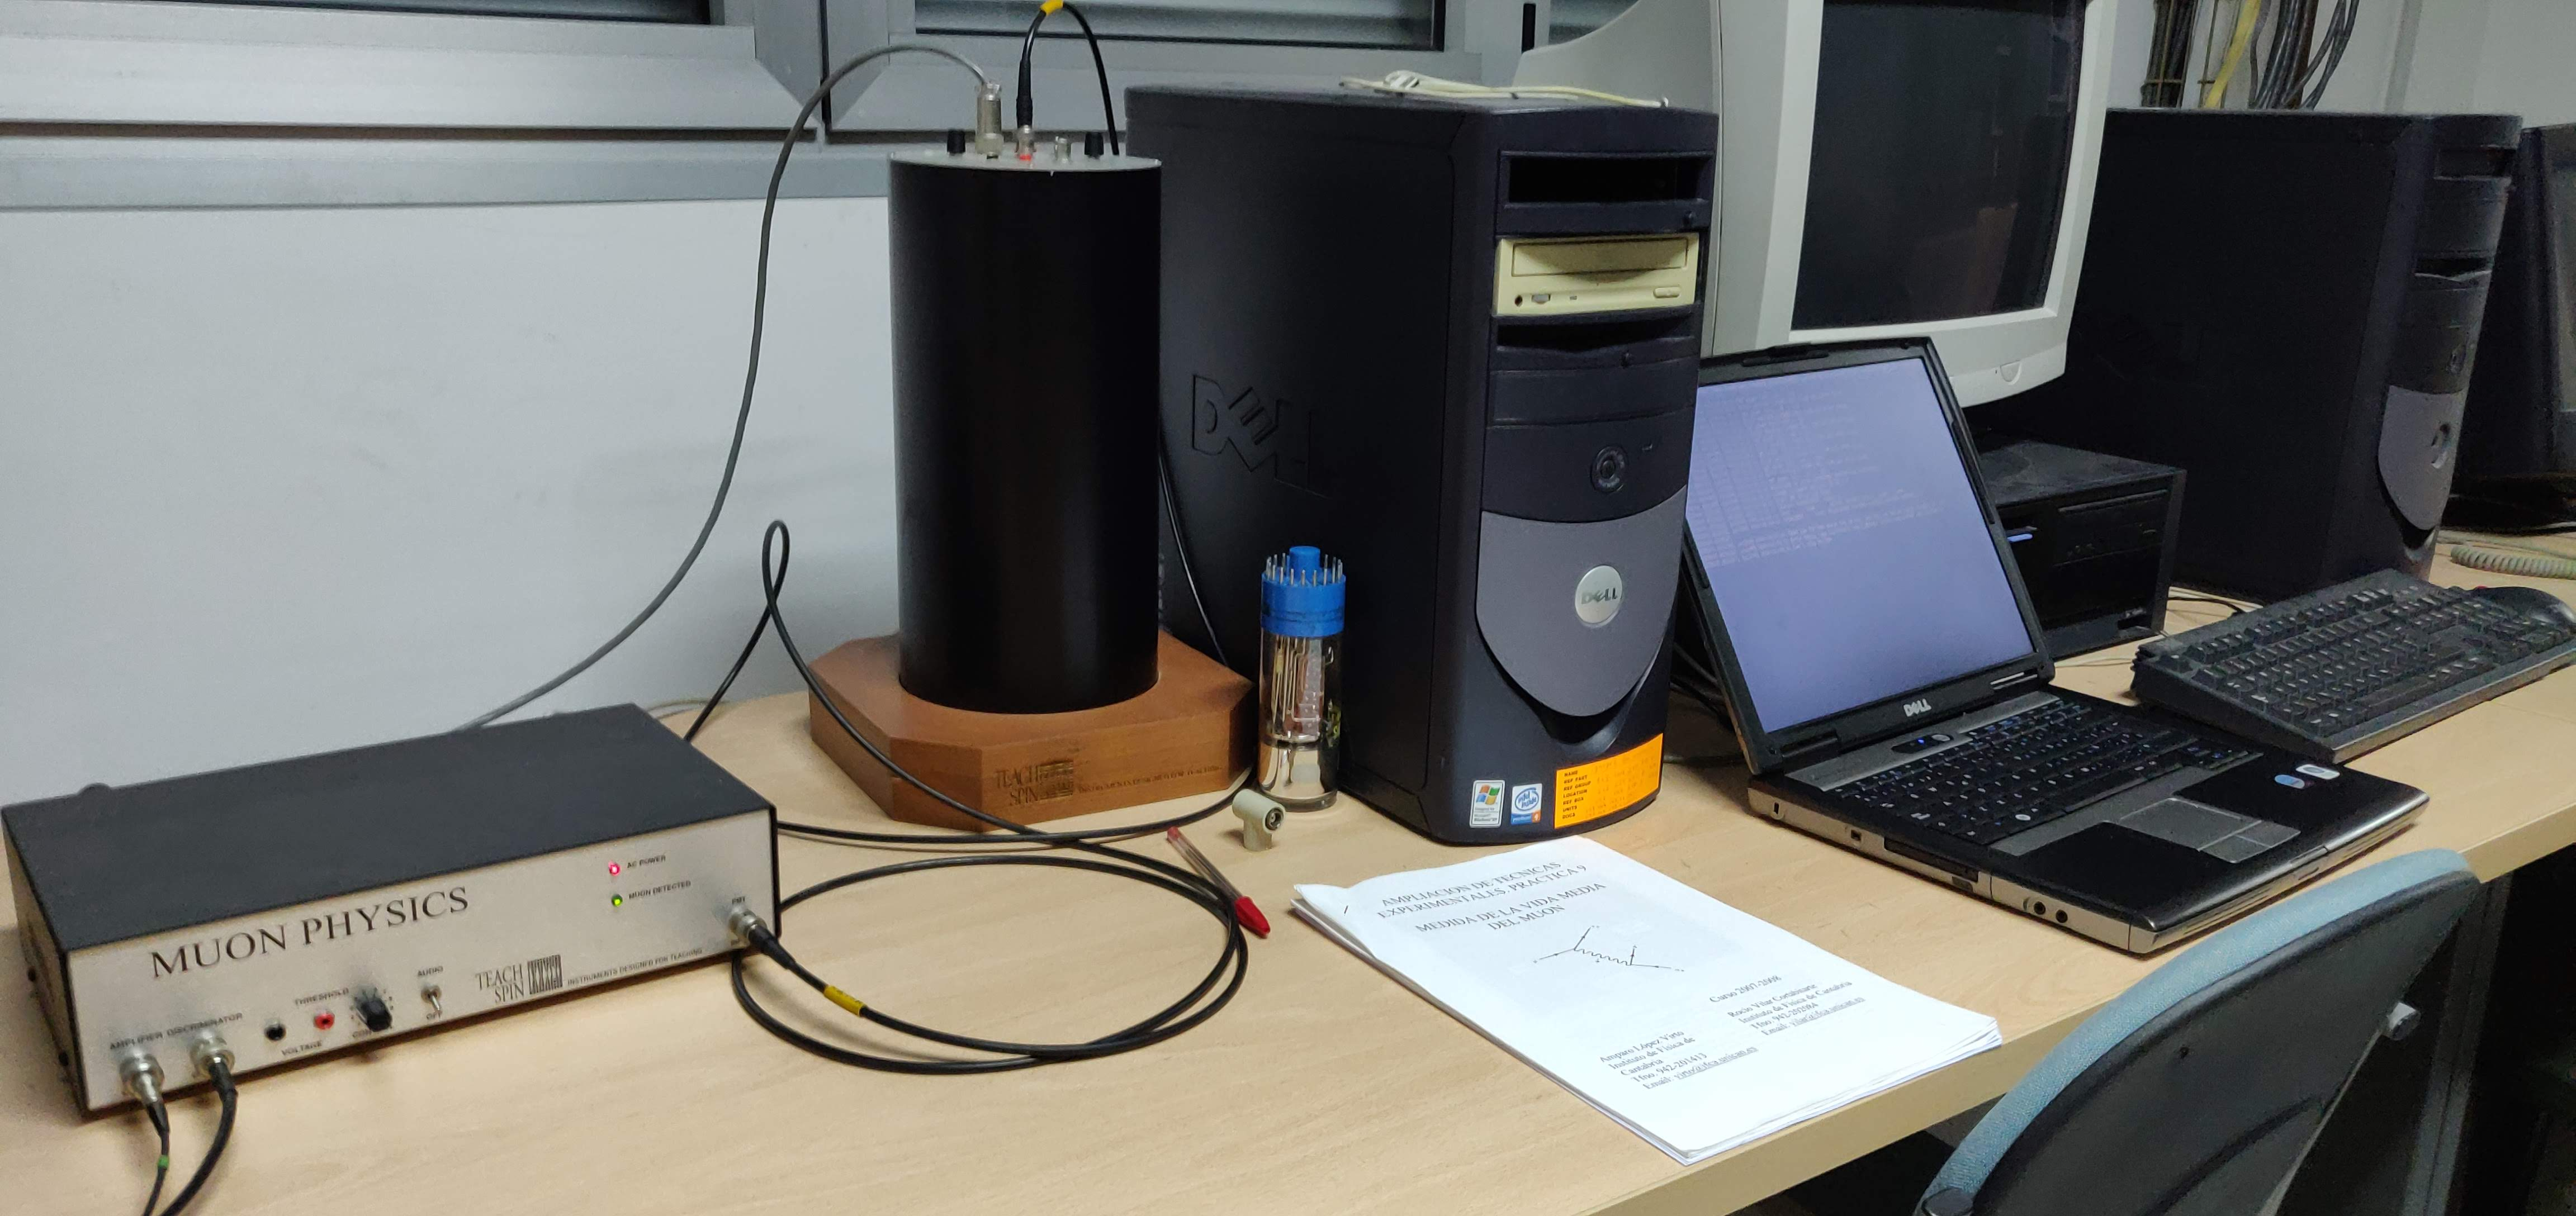
\includegraphics[scale=0.05]{Fotos/IMG_20180927_113646.jpg}
					\end{figure}
				}

				\only<1->{El experimento trabaja midiendo el tiempo de las desintegraciones de los muones recogidas en el detector.}
				\vspace{-0.75cm}

				\only<2->{

					\begin{multicols}{2}
						\[\mu^- \rightarrow e^- + \bar{\nu}_e + \bar{\nu}_\mu\]

						\begin{equation}
							P(t) = P(0)e^{-t/(\gamma \tau)}
						\end{equation}
					\end{multicols}
				}
			\end{frame}

			\subsection{Electrónica}

			\begin{frame}
				\frametitle{La Caja Electrónica de Lectura}

				\only<1->{

				\begin{minipage}[c]{0.6\linewidth}
					\begin{figure}[t]
						\centering
						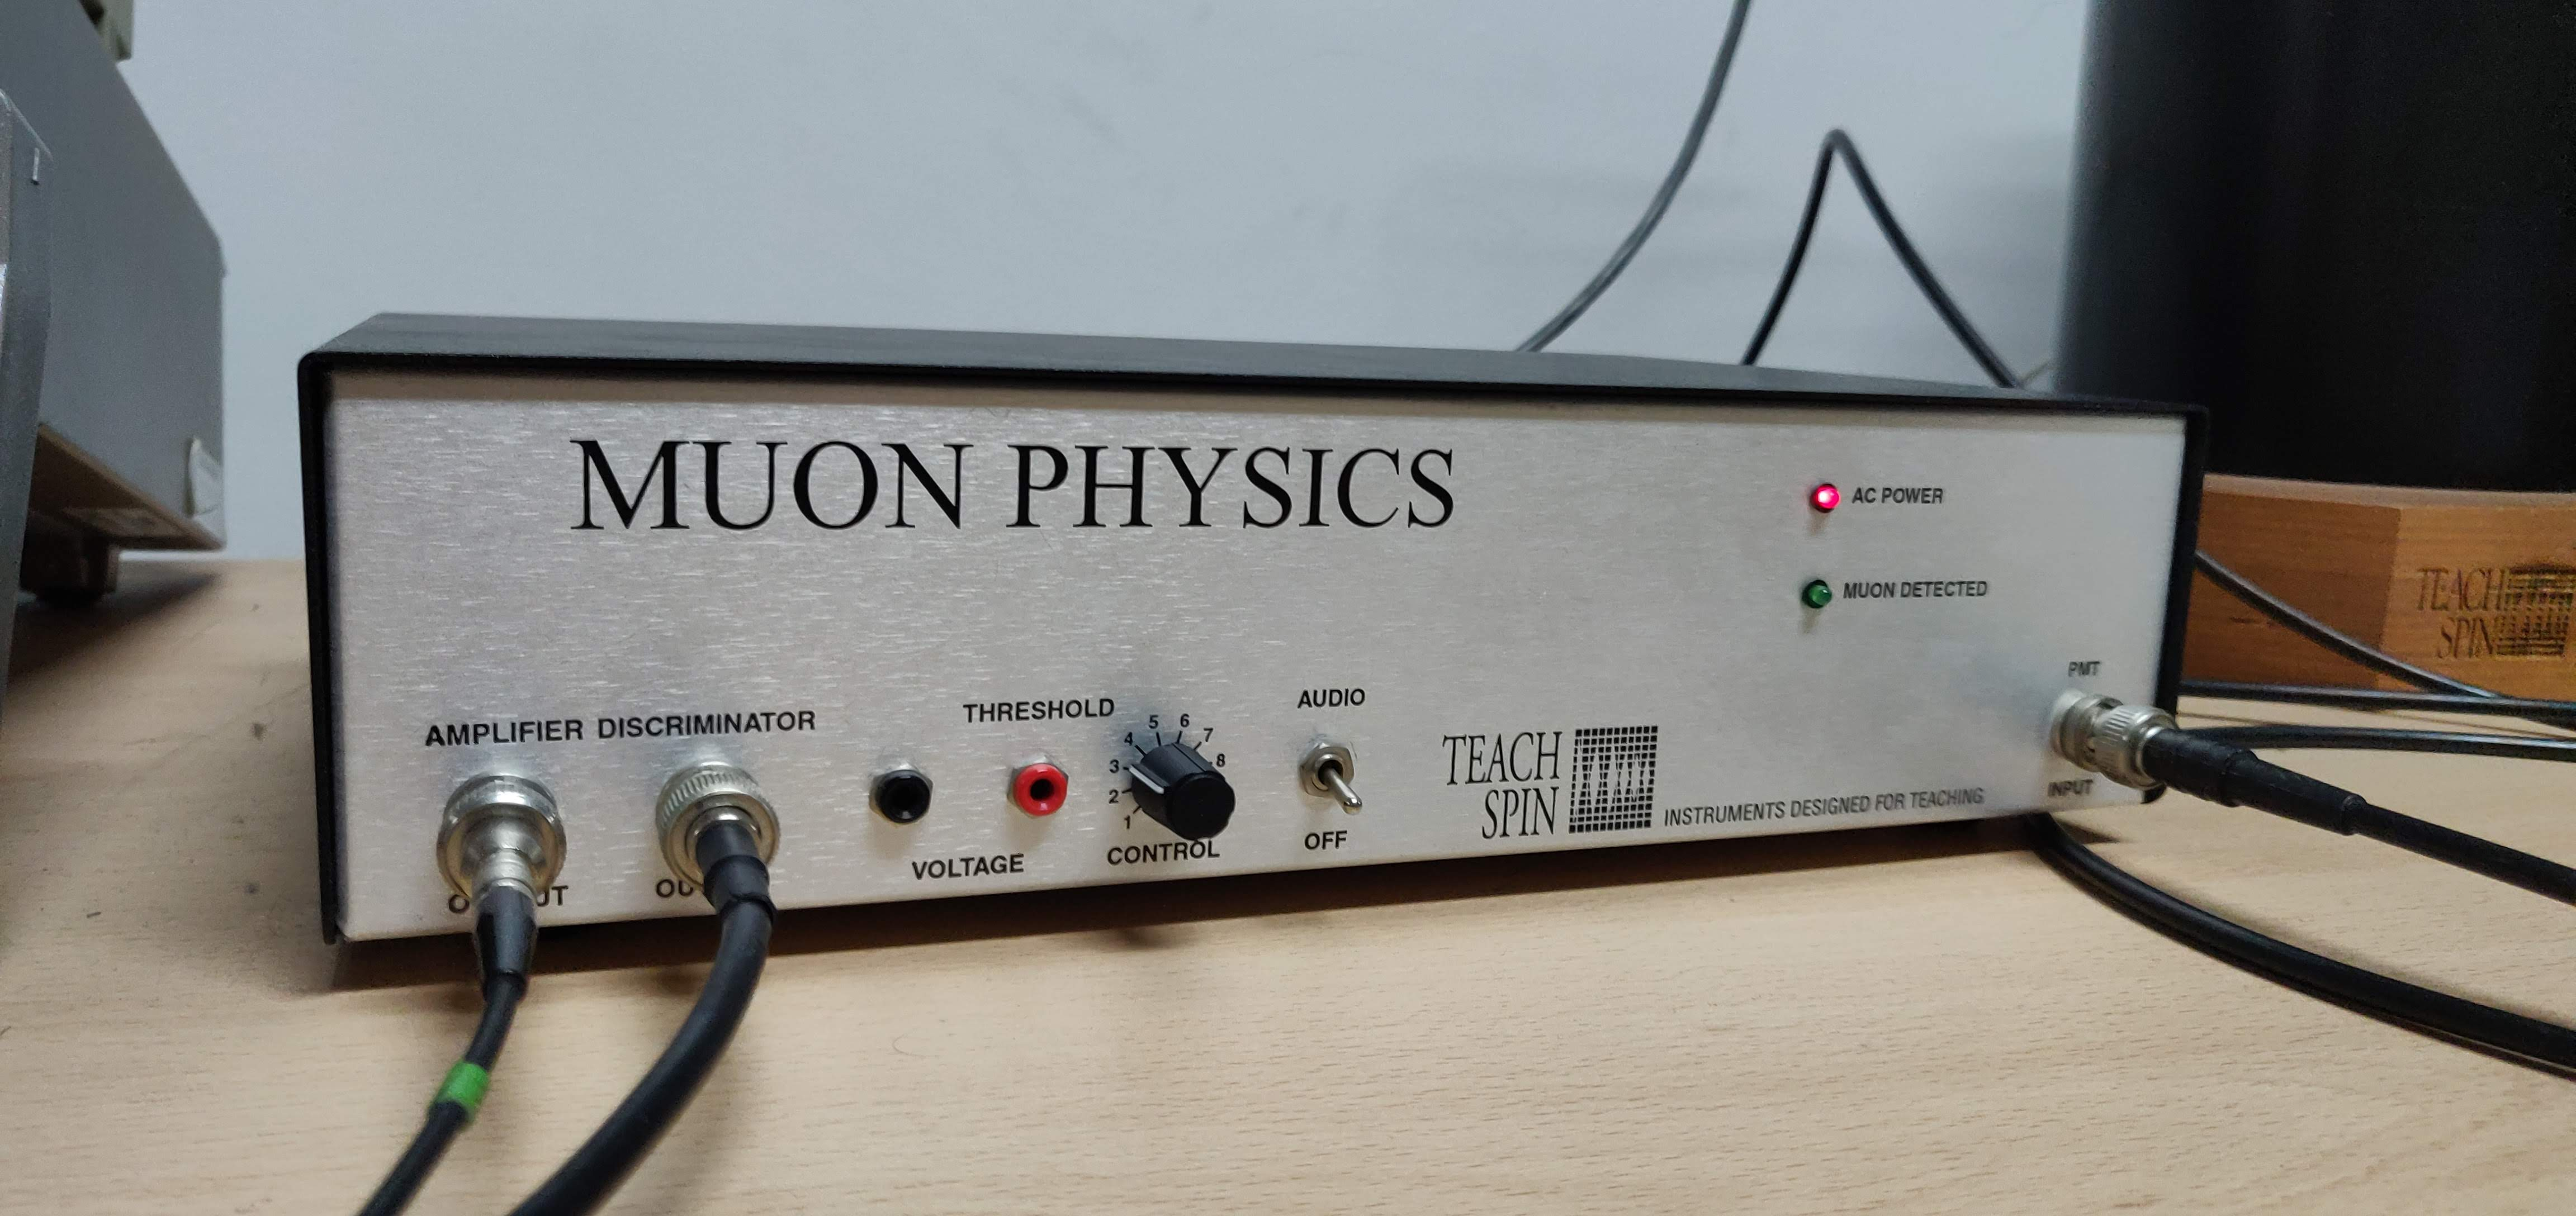
\includegraphics[scale=0.03]{Fotos/IMG_20180927_113549.jpg}
					\end{figure}

				\end{minipage}
				\begin{minipage}[c]{0.3\linewidth}
					Traduce las señales electricas del detector en tiempo de desintegración
					
				\end{minipage}

				}

				\only<2->{
				\begin{minipage}[c]{0.4\linewidth}

					\begin{equation*}
						20 \mu s = 1000 \cdot 50 MHz
					\end{equation*}

				\end{minipage}
				\begin{minipage}[c]{0.5\linewidth}

					\begin{figure}[b]
						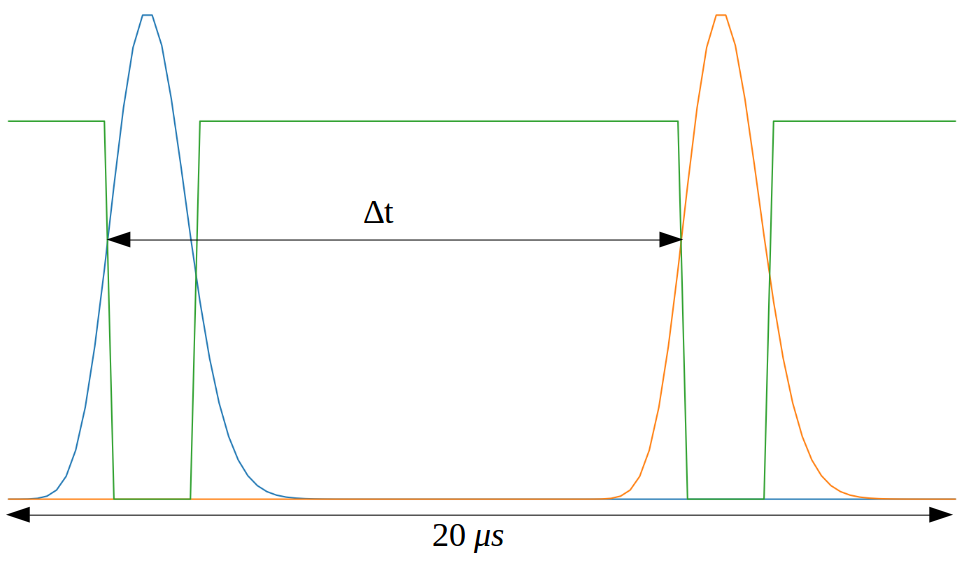
\includegraphics[scale=0.18]{Fotos/signalLabels.png}
					\end{figure}
				\end{minipage}}
			\end{frame}

		\section{El Software}

			\begin{frame}
				\frametitle{Esquema del Proceso del Programa}
				\begin{figure}[H]
					\centering
					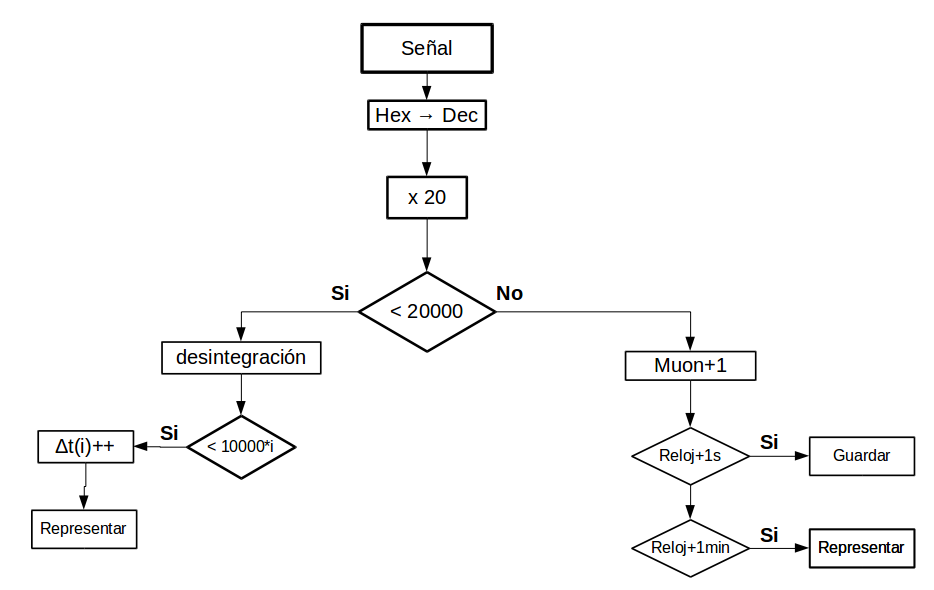
\includegraphics[scale=0.3]{Fotos/Esquema.png}
				\end{figure}
			\end{frame}

		\subsection{El Antiguo}

			\begin{frame}
				\frametitle{Desventajas del Antiguo Software}

					\begin{itemize}
						\item<1-> El software no ha sido actualizado desde su adquisición.

						\item<2-> Está escrito en el lenguaje de programación Tcl/Tk, poco común y desconocido.

						\item<3-> Actualmente solo está disponible para una versión antigua de Windows.

						\item<4-> El ajuste de los valores para la obtención del tiempo de mida media del muón se realiza teniendo en cuenta la función de probabilidad Gaussiana, en lugar de la Poissoniana propia de los histogramas como el del experimento.
					\end{itemize}
			\end{frame}

			\begin{frame}
				\frametitle{El Software del Fabricante}
				\begin{figure}[H]
					\centering
					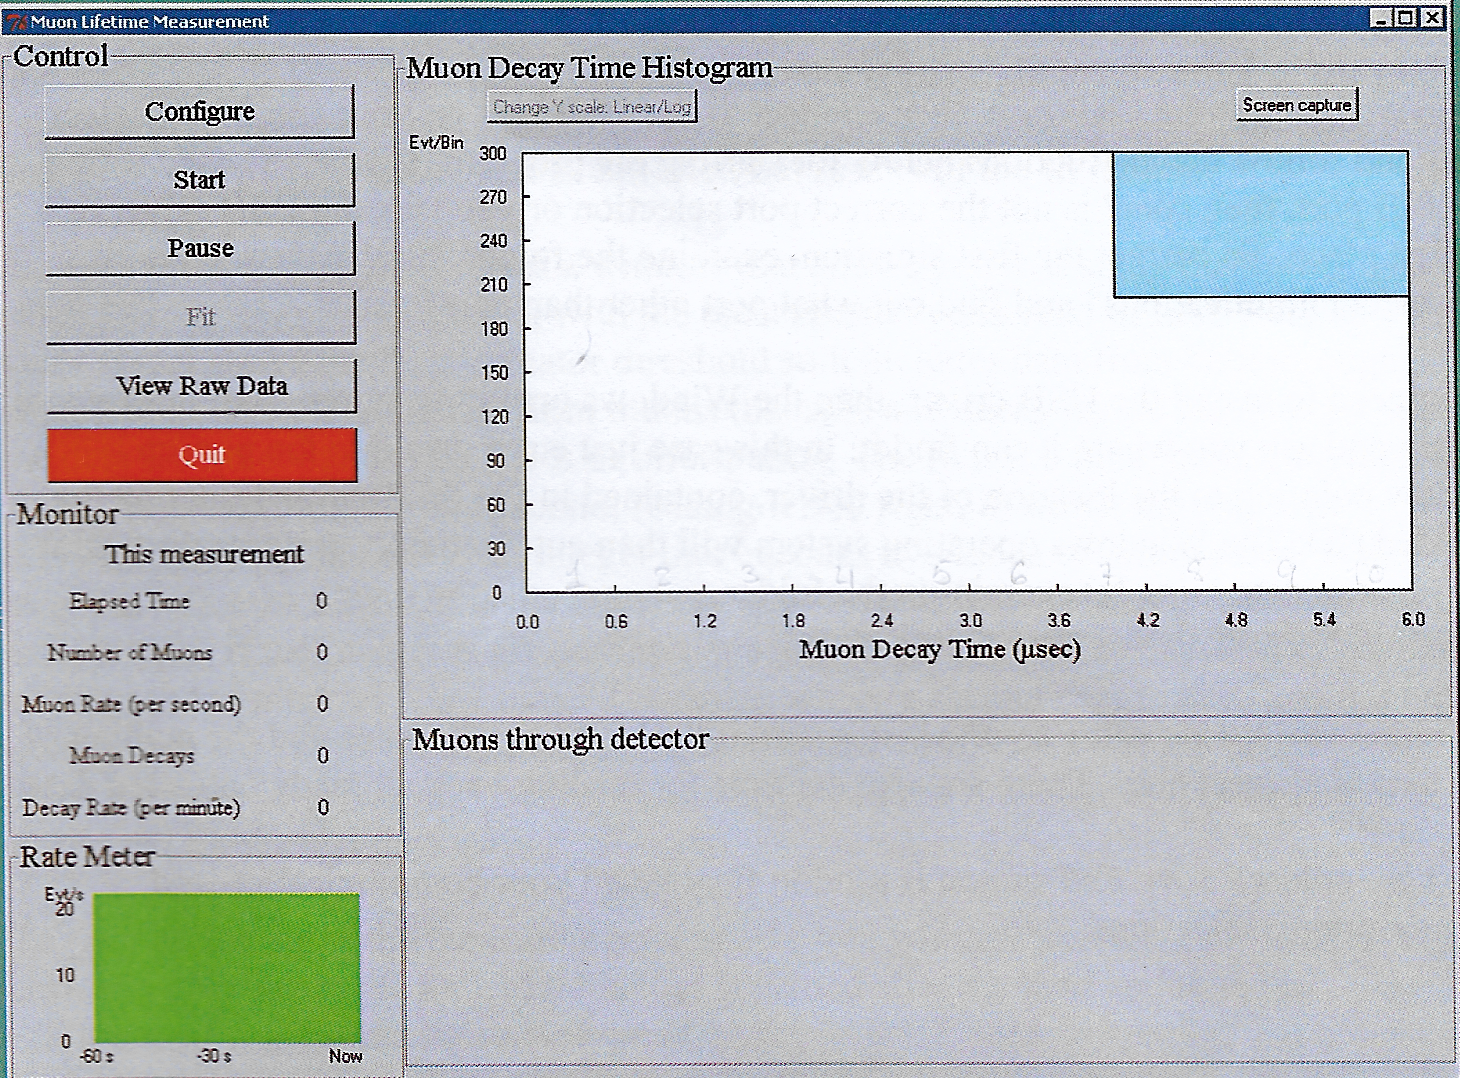
\includegraphics[scale=0.7]{Fotos/Scanned_Document.png}
				\end{figure}
			\end{frame}


		\section{MULTI-DAQ}

			\begin{frame}
				\frametitle{Propuestas del Nuevo Software}

					\begin{itemize}
						\item<1-> El nuevo software está escrito en el lenguaje C++ facilitando su actualización en el futuro y pudiendo ser compilado en diferentes ordenadores.

						\item<2-> Enfocado para sistemas Linux

						\item<3-> Interfaz en modo texto desarrollada usando Ncurses para poder ser usado de forma remota mediante ssh.

						\item<4-> El ajuste de la exponencial se realiza utilizando la librería ROOT teniendo en cuenta la distribución Poissoniana.

						\item<5-> Se ha añadido la opción de parar/reiniciar la toma de datos. 
					\end{itemize}
			\end{frame}

			\subsection{Interfaz del Programa}

			\begin{frame}
				\frametitle{Interfaz Gráfica de MULTI-DAQ}
					\centering

					\begin{figure}[H]
						\centering
						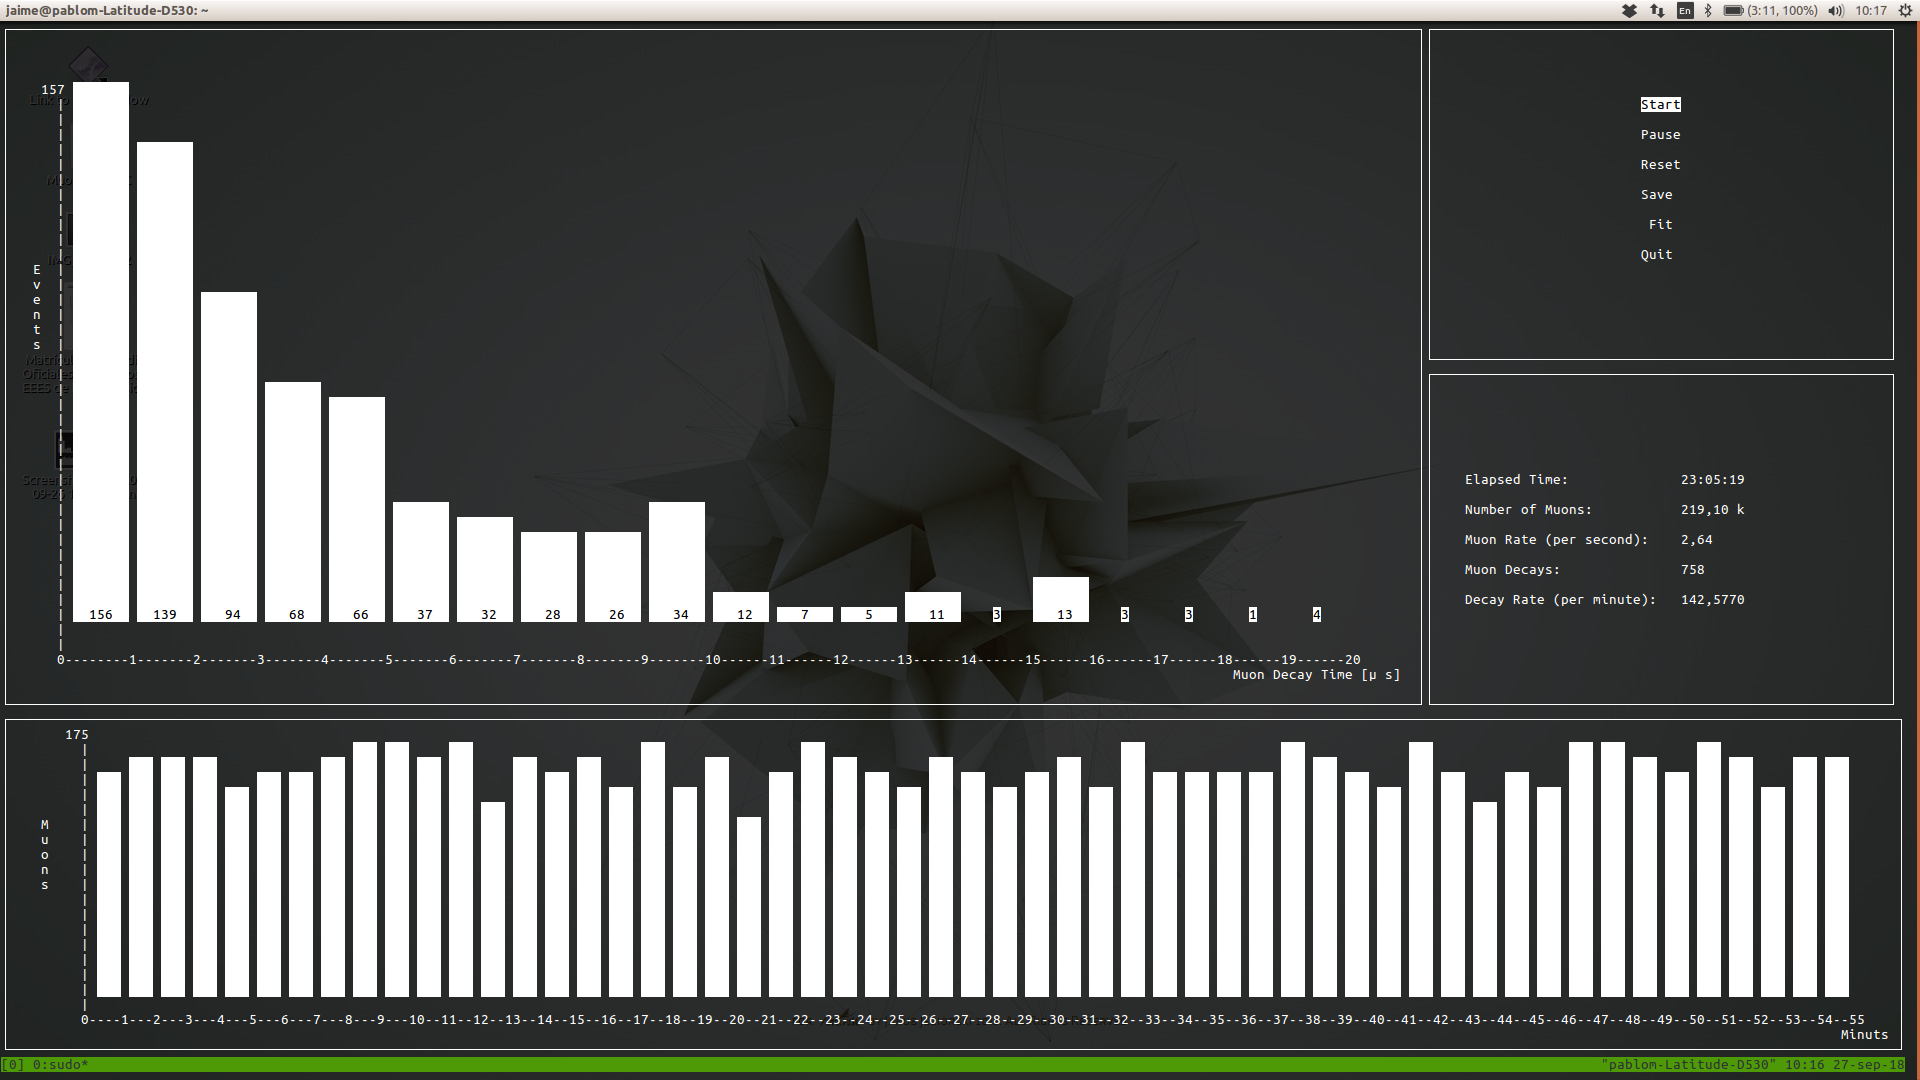
\includegraphics[scale=0.15]{Figuras/soooPerfect.png}
					\end{figure}

			\end{frame}

			\begin{frame}
				\frametitle{Guardar los Datos}

					\only<+->{Los datos son guardados en un archivo .txt con la fecha de la toma de datos, con el el tiempo obtenido del detector y la fecha en segundos del momento de la detección desde el 1 de Enero de 1970.}

					\only<+->{\begin{figure}[H]
						\centering
						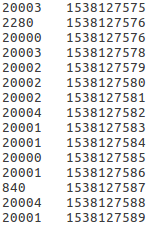
\includegraphics[scale=0.6]{Figuras/Data.png}
					\end{figure}}
			\end{frame}

			\subsection{Ajuste}

			\begin{frame}
				\frametitle{Ajuste de los datos}

				El ajuste se realiza definiendo la función $exp([0]+[1]*x)$ mediante la clase TF1 de ROOT.
				\begin{figure}[H]
					\centering
					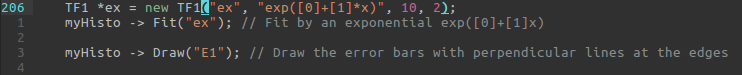
\includegraphics[scale=0.4]{Fotos/code.png}
				\end{figure}
			\end{frame}

			\begin{frame}
				\frametitle{Ajuste de los datos}

				\only<1->{

				\begin{minipage}[c]{0.7\linewidth}
					\begin{figure}[t]
						\centering
						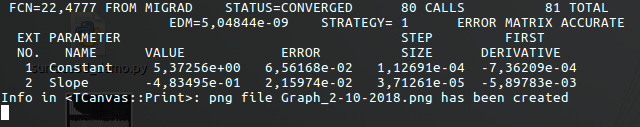
\includegraphics[scale=0.4]{Figuras/Fit.png}
					\end{figure}

				\end{minipage}
				

				}

				\only<2->{
				\begin{minipage}[c]{0.4\linewidth}

					\begin{equation*}
						\tau = \frac{-1} {p1} = \frac{1} {4.83495} 
					\end{equation*}
					\begin{equation*}
						\tau = (2.07 \pm 0.09) \mu s
					\end{equation*}

				\end{minipage}
				\begin{minipage}[c]{0.5\linewidth}

					\begin{figure}[b]
						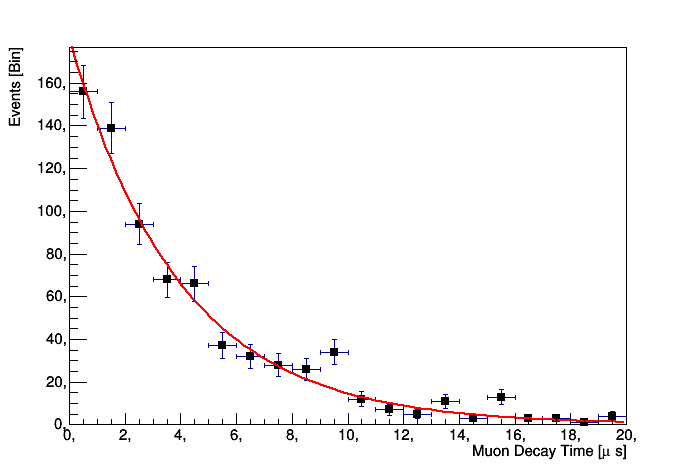
\includegraphics[scale=0.28]{Figuras/Graph_27-9-2018.png}
					\end{figure}
				\end{minipage}}
			\end{frame}

			\begin{frame}

				El código está dispoble en GitHub bajo licencia Creative Commons Attribution 4.0.

				\vspace{1cm}

				\url{https://github.com/Jaimedgp/Muon-Experiment-reader}
			\end{frame}

			\begin{frame}
				\centering
				\Huge

				So long \\ and \\ thanks for \\ all the fish

			\end{frame}

			

\end{document} 